\icode{E-MI-SI-L2-261110-001}
如图，细而轻的绳子的两端分别系有质量为的\(m_A\)、\(m_B\)两球（可视为质点），\(m\)静止在光滑的半球	形表面点，已知过\(P\)点的半径与水平面的夹角为\qty{60}{\degree}，则\(m_A\)和\(m_B\)的关系为\paren[]

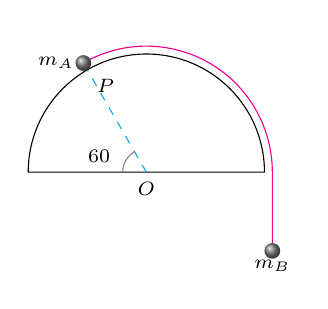
\begin{tikzpicture}[font=\scriptsize]
	\draw (-1.5,0) arc(180:0:1.5)--(-1.5,0);
	\draw[dashed,cyan] (0,0)node[below,black]{\(O\)}--(120:1.5)node[below right,black]{\(P\)};
	\draw[magenta] (120:1.6) arc(120:0:1.6)--(1.6,-1);
	\shade[ball color=gray] (120:1.6)node[left]{\(m_A\)} circle(.1);
	\shade[ball color=gray] (1.6,-1)node[below]{\(m_B\)} circle(.1);
	\draw[gray] (-.3,0) arc(180:120:.3);
	\node at(-.6,.2){\qty{60}{\degree}};
\end{tikzpicture}
\begin{choices}
	\item\(m_A = m_B\)
	\item\(m_A = \sqrt{3}m_B\)
	\item\(m_A = 2m_B\)
	\item\(m_A = \dfrac{\sqrt{3}}{3}m_B\)
\end{choices}
\begin{answer}
	C\qquad 提示：
\end{answer}